%%%%%%%%%%%%%%%%%%%%%%%% PREAMBLE
% \documentclass{beamer}
%%%%%%%%%%%%%%%%%%%%%%%% PREAMBLE
\documentclass[handout]{beamer}
\usepackage{pgfpages}
\usepackage{handoutWithNotes}
\pgfpagesuselayout{4 on 1 with notes}[a4paper,border shrink=5mm]
% \pgfpagesuselayout{4 on 1}[a4paper,border shrink=5mm]
%%%%%%%%%%%%%%%%%%%%%%%% PREAMBLE
\usepackage[T1]{fontenc}
\UseRawInputEncoding
\usepackage{graphicx, calligra}
\graphicspath{ {./figs/} }% other packages
\usepackage{latexsym,amsmath,xcolor,multicol,booktabs,calligra}
\usepackage{graphicx,listings,stackengine}
\usepackage{BGU}
\usepackage{todonotes}
\presetkeys{todonotes}{inline}{}

% defs
\def\cmd#1{\texttt{\color{red}\footnotesize $\backslash$#1}}
\def\env#1{\texttt{\color{blue}\footnotesize #1}}
\definecolor{deepblue}{rgb}{0,0,0.5}
\definecolor{deepred}{rgb}{0.6,0,0}
\definecolor{deepgreen}{rgb}{0,0.5,0}
\definecolor{halfgray}{gray}{0.55}

\lstset{
    basicstyle=\ttfamily\small,
    keywordstyle=\bfseries\color{deepblue},
    emphstyle=\ttfamily\color{deepred},    % Custom highlighting style
    stringstyle=\color{deepgreen},
    numbers=left,
    numberstyle=\small\color{halfgray},
    rulesepcolor=\color{red!20!green!20!blue!20},
    frame=shadowbox,
}

%%%%%%%%%%%%%%%%%%%%%%%% BEAMER NOTES
% https://gist.github.com/andrejbauer/ac361549ac2186be0cdb
% These slides also contain speaker notes. You can print just the slides,
% just the notes, or both, depending on the setting below. Comment out the want
% you want.

\setbeameroption{hide notes} % Only slides
%\setbeameroption{show only notes} % Only notes
% \setbeameroption{show notes on second screen=right} % Both

% To give a presentation with the Skim reader (http://skim-app.sourceforge.net) on OSX so
% that you see the notes on your laptop and the slides on the projector, do the following:
% 
% 1. Generate just the presentation (hide notes) and save to slides.pdf
% 2. Generate only the notes (show only nodes) and save to notes.pdf
% 3. With Skim open both slides.pdf and notes.pdf
% 4. Click on slides.pdf to bring it to front.
% 5. In Skim, under "View -> Presentation Option -> Synhcronized Noted Document"
%    select notes.pdf.
% 6. Now as you move around in slides.pdf the notes.pdf file will follow you.
% 7. Arrange windows so that notes.pdf is in full screen mode on your laptop
%    and slides.pdf is in presentation mode on the projector.

% Give a slight yellow tint to the notes page
\setbeamertemplate{note page}{\pagecolor{yellow!5}\insertnote}\usepackage{palatino}


%%%%%%%%%%%%% BEAMER SETTINGS %%%%%%%%%%%%%%
% \AtBeginSection[]
% {
% \begin{frame}<beamer>
% \frametitle{Plan}
% \tableofcontents[currentsection]
% \end{frame}
% }

% \AtBeginSubsection[] % Do nothing for \subsection*
% {
% % \begin{frame}<beamer>
% % \frametitle{Outline}
% % \tableofcontents[currentsection,currentsubsection]
% % \end{frame}
% }

%%% MACROS
\usepackage{svg}
\usepackage{pdfpages}
\usepackage{amsmath}
\usepackage{bm}
\newcommand{\policy}{\ensuremath{\boldsymbol{\pi}}}

\theoremstyle{definition}
% \newtheorem{definition}{Definition}[section]

% Allows repeating frame contents (duplicating boxes)
% https://tex.stackexchange.com/questions/107237/repeating-frame-contents
\newcommand\dupbox[2][]{%
\begin{block}{\duptitle}
\begin{minipage}{\linewidth}
\duptext
\end{minipage}
\end{block}
\begin{block}{#1}
\begin{minipage}{\linewidth}
#2
\end{minipage}
\end{block}
\gdef\duptext{#2}
\gdef\duptitle{#1}
}

\gdef\duptext{Initial text}
\gdef\duptitle{}



%%%%% THEME
% \usetheme{Boadilla}
% \usetheme{Madrid}
% \usecolortheme{default}


%%%% HEADER
\title[Probabilistic Inference for Solving MDPs]{Probabilistic Inference for Solving \\Markov Decision Processes}
\subtitle{Toussaint, Storkey, ICML '06}
\author{Noam Siegel}
\institute[BGU]
{Computer Science M.Sc. Seminar\\
Ben Gurion University}
\date{\today}


%%%%%%%%%%%%% DOCUMENT %%%%%%%%%%%%%%
\begin{document}

%%%%%%%%%%%%% Title Page %%%%%%%%%%%%%%

\begin{frame}
	\titlepage
	\note[item]{Thank the audience for being awake.}
	\note[item]{Prepare markers.}
	\note[item]{Start the timer.}
\end{frame}


%%%%%%%%%%%%% TOC %%%%%%%%%%%%%%
\begin{frame}
	\frametitle{Outline}
	\tableofcontents
\end{frame}

%%%%%%%%%%%%% DOCUMENT %%%%%%%%%%%%%%
\section{Introduction}

%%%%%%%%%%%%% Preliminaries %%%%%%%%%%%%%%

% \subsection{Prerequisites}

% \begin{frame}{Prerequisites}
%         \todo{todo: add prerequisites}
% % 		\todo{add illustration of Probabilistic Inference in Graphical Models}
% % 		\todo{add illustration of Dynamic Bayesian Networks}
%         \note{for example: probabilistic inference, graphical models, dynamic bayesian networks}
% \end{frame}

%%%%%%%%%%%%% Problem %%%%%%%%%%%%%%
\subsection{Getting started}
\begin{frame}<1-3>{Getting started}
    \setbeamercolor{background canvas}{bg=}
    \only<1>{
    \includegraphics[width=\textwidth]{figs/fig_0a_starting.png}
    }
    \only<2>{
    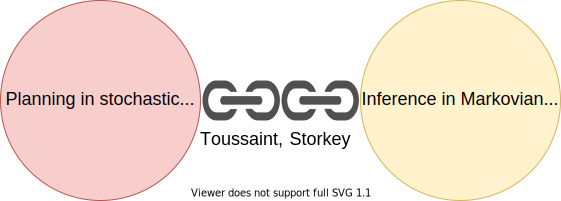
\includegraphics[width=\textwidth]{figs/fig_0b_starting.png}
    % 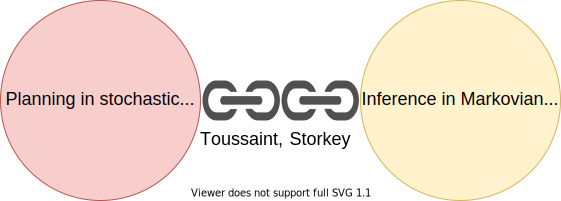
\includepdf[]{figs/fig_0b_starting.pdf}
    }
    \only<3>{
    \begin{enumerate}
        \item \emph{Bui et al. (2002)} have used inference on Abstract Hidden Markov Models for policy recognition, but not for computing an optimal policy.
        \item \emph{Attias (2003)} got close to translating the problem of planning to a problem of inference. Here, however, the total time $T$ has to be fixed \emph{ad hoc} and the MAP action sequence that is proposed as a solution is not optimal.
        \item \emph{Verma and Rao (2006)} used inference to compute plans, but again the total time has to be fixed and the plan is not optimal.
    \end{enumerate}
    }
% 	\begin{itemize}
% 		\item Factored Markov Decision Processes
% 		\item Approximate inference on factorial latent representations
% 		\item Abstract Hidden Markov Models
% 		\item Attias (2003)
% 		\item Verma and Rao (2006)
% 	\end{itemize}
	\note[item]{The paper I am presenting to you bridges beautifully between two fields: planning in stochastic environments, and inference in Markovian models.}
	\note[item]{discuss similarities between fields: both face the challenge of coping with very large state spaces spanned by multiple state variables, or realizing planning (or inference) in continuous state spaces.}
	\note[item]{cite existing ways to deal with challenges in each field: Factored MDPs or abstractions (in planning), approximate inference (inference).}
	\note[item]{describe and mention previous approaches to merging planning and inference, and mention their limitations.}
	\note[item]{For related work: Not optimal in the sense of maximizing an expected future reward}
\end{frame}


\subsection{Main contribution}
\begin{frame}{Main contribution}
	\begin{block}{Contribution}
		\begin{enumerate}
			\item<1-> Translate the problem of maximizing the expected future return exactly into a problem of likelihood maximization in a latent variable model, for arbitrary reward functions and episode length.
			\item<2-> Demonstrate the approach on a discrete problem, then on a continuous stochastic optimal control problem.
		\end{enumerate}
	\end{block}
	\note<1>[item]{item1: provide a framework that translates the problem of maximizing the expected future return exactly into a problem of likelihood maximization in a latent variable mixture model, for arbitrary rewards functions and without assuming a fixed time}
	\note<2>[item]{item2: demonstrate the approach first on a discrete maze problem using exact inference in the E-step, then on a continuous stochastic optimal control problem assuming Gaussian belief state representations and using the unscented transform to handle non-linear dynamics.}
	\note[item]{The key step to our approach is to introduce a mixture of finite-time MDPs as a model that is equivalent to the original time-unbounded MPD but has two advantages: it allows us to formulate a likelihood proportional to the expected future return, and inference in the mixture model can efficiently be realized with a single synchronous forward-backward propagation without having to fix a finite total time in advance.}
\end{frame}


\section{Research Problem}

\subsection{Markov Decision Processes}
% \makeatletter
% \newenvironment{myalign}{%
%   \setlength{\abovedisplayskip}{-\baselineskip}%
%   \setlength{\abovedisplayshortskip}{\abovedisplayskip}%
%   \start@align\@ne\st@rredtrue\m@ne
% }%
% {\endalign}
% \makeatother

\begin{frame}<1-3>{Markov Decision Processes}
	\only<1,2>{
	\includegraphics[width=\textwidth]{figs/fig_1_dbn_mdp.png}
	}
	\only<2,3>{
	\begin{definition}[MDP]
		\begin{smashedalign}
			\text{state transition probability } &P(x_{t+1} \mid a_t, x_t)\\
			\text{action probability } &P(a_t \mid x_t; \policy)\\
			\text{reward probability } &P(r_t \mid a_t; x_t), \quad \quad r_t \in \{0, 1\}
		\end{smashedalign}
	\end{definition}
	}
	\only<3>{
	\begin{definition}[Policy \policy{}]
	    The action probabilities are parameterized by a policy:
	    \begin{equation*}
	         P(a_t \mid x_t = i; \policy) = \pi_{ai} \quad \quad s.t. \sum_a \pi_{ai} = 1
	    \end{equation*}
	\end{definition}
	}
	\note[item]{Throughout this paper we assume that the transition and reward probabilities are given, i.e. known a priori. Such probabilities can be estimated from experience, but this is not addressed here.}
	\note[item]{The random variables $x$ and $a$ can be discrete or continuous}
	\note[item]{The reward variable $r$ is, w.l.g. assumed to be binary, $r_t \in \{0, 1\}$}
	\note[item]{The action probability $P(a_t \mid x_t ; \policy)$ is directly parameterized by an unknown policy \policy{} such that $P(a$}
	\note[item]{in case asked: w.l.g.: Assuming binary reward variables is sufficient to associate arbitrary reward expectations $P(r_t \mid a_t, x_t)$ in the interval $[0,1]$ to states and actions, which is, modulo rescaling, the general case in Reinforcement Learning scenarios.}
	\note{DRAW Figure 1 on the board!}
\end{frame}


\begin{frame}{Research problem}
	\begin{definition}[solving an MDP]
	\label{def:solve_mdp}
		\emph{Solving an MDP} means to find a parameter $\policy$ of the graphical model in Figure 1 that maximizes the expected future return $V^{\policy}(i) = E\{\sum_{t=0}^\infty \gamma^t r_t \mid x_0=i ; \policy \}$, where $\gamma \in [0, 1]$ is a discount factor.
	\end{definition}
	\pause
	\begin{alertblock}{research problem}
	The problem is to \emph{solve the MDP}, i.e. to find a policy that maximizes the expected future return.
	\end{alertblock}
	\note<1>[item]{This definition is an equivalent definition to the standard definition, since reductions can be made in both directions.}
	\note<2>[item]{The problem is to \emph{solve the MDP}, i.e., to find a policy that maximizes the expected future return}
	\note<2>[item]{The classical approach to solving MDPs is anchored in Bellman's equation, which simply reflects the recursive property of the future discounted return $R_T = \sum_{t=T}^{\infty} \gamma^t r_t = r_T + \gamma R_{T+1}$ and consequently of its expectation conditioned on the current state, $V_{\policy} = \sum_{j,a} P(j \mid a, i) P(a \mid i ; \policy) [P(r_t = 1 \mid a, i) + \gamma V^{\policy}(j)]$.}
	\note<2>[item]{Standard algorithms for computing value functions can be viewed as iterative schemes that converge towards the Bellman equation.}
	\note{WRITE $V^{\policy}(i) = E\{\sum_{t=0}^\infty \gamma^t r_t \mid x_0=i ; \policy \}$ on the board}
\end{frame}

\section{Research Plan}

\subsection{Mixture of MDPs and likelihood}
% \begin{frame}[shrink]{Mixture of MDPs}
% \includegraphics{figs/fig_2_mixture_mdps.png}
% \end{frame}

\makeatletter
\frame{{Mixture of MDPs}
	\global\beamer@shrinktrue
	\gdef\beamer@shrinkframebox{
		\setbox\beamer@framebox=\vbox to\beamer@frametextheight{
			\centering
			\includegraphics[height=\beamer@frametextheight]{figs/fig_2_mixture_mdps.png}
		}
	}
	\note[item]{Our approach is to cast the problem of solving an MDP into a problem of optimizing the parameters of a graphical model with many hidden variables, namely all future states and actions.}
	\note[item]{The only observables are the current state and rewards}
	\note[item]{To achieve exact equivalence between solving the MDP and standard likelihood maximization we will need to define a likelihood that is proportional to the expected future return.}
	\note[item]{This is most easily done by considering a \emph{mixture of finite-time MDPs}.}
	\note[item]{By a finite-time MDP we mean one which is limited in time by T, and which emits a reward variable only at the very final time step, as illustrated for various T in figure 2.}
	\note{DRAW Figure 2. on the board!}
}
\makeatother

\begin{frame}{Representing the joint distribution $P(\mathcal{X})$}
	\begin{block}{full joint for finite time MDP}
		\begin{smashedalign}
			  & P(r, x_{0:T}, a_{0:T} \mid T ; \policy) = \\& P(r \mid a_T, x_T)P(a_0 \mid x_0 ; \policy) P(x_0) \cdot \prod_{t=1}^{T}{P(a_t \mid x_t ; \policy) P(x_t \mid a_{t-1}, x_{t-1}})
		\end{smashedalign}
		
	\end{block}
	\pause
	\begin{block}{full joint for mixture of finite-time MDPs}
		$P(r,x_{0:T}, a_{0:T}, T ; \policy) = P(r, x_{0:T}, a_{0:T} \mid T ; \policy) P(T)$
	\end{block}
	\pause
	\begin{block}{prior over the total time}
	$P(T) = \gamma^T(1-\gamma)$
	\end{block}
	
	
	\note[item]<1>{This reads: The probability of seeing a reward $r$, a state sequence $x_{0:T}$, and an action sequence $a_{0:T}$, given an episode length $T$ and a policy $\policy$, can be factored into multiple conditional probabilities. This means we can write it down as a product of the probability of seeing a reward $r$ conditioned on the final state $x_T$ and action $a_T$, the probability of performing an action $a_0$ at state $x_0$ under policy $\policy$, the probability of observing state $x_0$, and for each $t \in \{1, .., T\}$ the probability of performing action $a_t$ at state $x_t$ under policy $\policy$, times the probability of transitioning from $x_{t-1}$ to $x_t$ if the action performed was $a_{t-1}$.}
	\note[item]<2>{This reads: using the chain rule, the joint probability of the observed reward, state sequence and action sequence, at a general time T, parameterized by the policy $\policy$, is a product of the full joint for finite time MDP, and the prior probability we associate with the time variable $T$..}
	\note[item]<3>{Here, $P(T)$ is a prior over the total time, which we choose proportional to the discounting.}
	\note[item]<3>{Note that each finite-time MDP shares the same transition probabilities and is parameterized by the same policy $\policy$}
	\note<3->{DRAW P(T) on board}
\end{frame}

\begin{frame}{Defining the likelihood}
    \begin{definition}[likelihood for a finite-time MDP]
        $L_T^{\policy}(i) = P(r=1 \mid x_0=i, T ; \policy) = E\{r \mid x_0 = i, T ; \policy\}$
    \end{definition}
    \pause
    \begin{definition}[likelihood for mixture of MDPs]
        $L^{\policy}(i) = P(r = 1 \mid x_0 = i; \policy) = \sum\limits_T P(T)E\{r \mid x_0 = i, T ; \policy\}$
    \end{definition}
    \pause
    \begin{corollary}
        $L_T^{\policy}(i) = (1 - \gamma) V^{\policy}(i)$
    \end{corollary}
    \note<1->[item]{Each time-bounded MDP allows us to formulate a likelihood proportional to the expected future return for that run.}
    \note<2->[item]{The mixture of time-bounded MDPs allows us a likelihood proportional to the expected future return for any run, regardless of the episode length.}
    \note<3->[item]{This likelihood is, for the discounted time prior $P(T) = \gamma^T(1-\gamma)$, proportional to the expected future return.}
    \note<3->[item]{Note that the expectation term $E\{r \mid x_0 = i, T; \policy\}$ here is exactly the same as the terms $E\{r_t \mid x_0 = i ; \policy\}$ for $t=T$ in definition \ref{def:solve_mdp}: we are taking the expectation w.r.t. a full probabilistic forward-sweep through the MDP, from time 0 to time T, given the policy \policy. All MDPs share the same transition probabilities}
\end{frame}

\begin{frame}{Theoretical Guarantee}
	\begin{block}{Reminders}
	    \begin{enumerate}
	        \item \emph{Solving an MDP} means to find a parameter $\policy$ of the graphical model in Figure 1 that maximizes the expected future return $V^{\policy}(i) = E\{\sum_{t=0}^\infty \gamma^t r_t \mid x_0=i ; \policy \}$.
	        \item The \emph{likelihood for a mixture of MDPs} is given by $L^{\policy}(i) = P(r = 1 \mid x_0 = i; \policy) = \sum\limits_T P(T)E\{r \mid x_0 = i, T ; \policy\}$
	        \item This implies that $L_T^{\policy}(i) = (1 - \gamma) V^{\policy}(i)$
	    \end{enumerate}
	\end{block}
    \pause
    \begin{theorem}
        Maximizing the likelihood in the mixture of finite-time MDPs is equivalent to solving the MDP.
    \end{theorem}
    \note<1->[item]{Let us remember what we've seen so far.}
    \note<2->[item]{Thus, we have establised an important theoretical guarantee: there is an exact equivalence between the maximization of the likelihood and expected future return.}
    \note<2->[item]{Note that considering the mixture of finite-time models has a second advantage: the finite-time property of every mixture component makes the E-step in the full mixture model rather simple and efficient, as detailed in the next section.}
\end{frame}


\subsection{An EM-algorithm for computing the optimal policy}
\begin{frame}{An EM-algorithm for computing the optimal policy}
	\todo{Introduction to EM algorithms}
	
	\note[item]{Formulating the objective function in terms of a likelihood allows us to apply Expectation-Maximization to find optimal parameters (the policy \policy) of our model. All action and state variables (except for $x_0$ are hidden variables).}
	\note[item]{The E-step will, for a given $\policy$, compute posteriors over state-action sequences as well as $T$ conditioned on $x_0 = A$ and $r=1$}
	\note[item]{The M-step then adapts the model parameters $\policy$ to optimize the expected likelihood (expectations then taken w.r.t. the posteriors calculated in the E-step.}
	\note[item]{Conceptually, the E-step in this Markovian model is straight-forward. However, the special structure of the finite-time MDPs will allow for certain simplifications and save us from performing separate inference sweeps in all finite-time MDPs}
\end{frame}

\begin{frame}<1-4>{E-step: forward-backward in all MDPs synchronously}
    \only<1>{
    \begin{block}{Simplifying notation}
       \begin{enumerate}
        \item $p(j \mid a, i) = P(x_{t+1} = j \mid a_t = a, x_t = i)$
        \item $p(j \mid i; \policy) = P(x_{t+1} = j \mid x_t = i ; \policy) = \sum_a p(j \mid a, i) \pi_{ai}$
    \end{enumerate}  
    \end{block}
    }
    
    \only<2,3>{
    % \begin{definition}["seed" for backward propagation]
    % $\hat{\beta}(i) = P(r = 1 \mid x_T = i ; \policy) = \sum\limits_a P(r=1 \mid a_T=a, x_T = i) \pi_{ai}$
    % \end{definition}
    
    \begin{block}{Forward Propagation}
        \begin{columns}[b]
               \begin{column}{3cm}
                       $\alpha_0(i) = \delta_{i=A}$
               \end{column}
               \begin{column}{7cm}
                \begin{smashedalign}
                    \alpha_t(i) &= P(x_t=i \mid x_0 = A ; \policy)\\
                        &= \sum\limits_j p(i \mid j ; \policy) \alpha_{t-1}(j)
                \end{smashedalign}
               \end{column}
        \end{columns}
    \end{block}
    }
    \only<3->{
    \begin{block}{Backward Propagation (temp.)}
        \begin{columns}[b]
               \begin{column}{3cm}
                       $\tilde{\beta}_T(i) = \hat{\beta}(i)$
               \end{column}
               \begin{column}{7cm}
                \begin{smashedalign}
                    \tilde{\beta}_t(i) &= P(r = 1 \mid x_t = i ; \policy)\\
                        &= \sum\limits_j p(j \mid i ; \policy) \tilde{\beta}_{t+1}(j)
                \end{smashedalign}
               \end{column}
        \end{columns}
        Where $\hat{\beta}(i) = P(r = 1 \mid x_T = i ; \policy) = \sum\limits_a P(r=1 \mid a_T=a, x_T = i) \pi_{ai}$
    \end{block}
    }
    
    % \only<4->{
    % \begin{block}{Backward Propagation (temp.)}
    %     \begin{columns}[b]
    %           \begin{column}{3cm}
    %                   $\tilde{\beta}_T(i) = \hat{\beta}(i)$
    %           \end{column}
    %           \begin{column}{7cm}
    %             \begin{smashedalign}
    %                 \tilde{\beta}_t(i) &= P(r = 1 \mid x_t = i ; \policy)\\
    %                     &= \sum\limits_j p(j \mid i ; \policy) \tilde{\beta}_{t+1}(j)
    %             \end{smashedalign}
    %           \end{column}
    %     \end{columns}
    %     Where $\hat{\beta}(i) = P(r = 1 \mid x_T = i ; \policy) = \sum\limits_a P(r=1 \mid a_T=a, x_T = i) \pi_{ai}$
    % \end{block}
    % }
    \only<4>{
    \begin{block}{Backward Propagation (corrected)}
        \begin{columns}[b]
               \begin{column}{3cm}
                       $\beta_0(i) = \hat{\beta}(i)$
               \end{column}
               \begin{column}{7cm}
                \begin{smashedalign}
                    \beta_\tau(i) &= P(r = 1 \mid x_{T - \tau} = i ; \policy)\\
                        &= \sum\limits_j p(j \mid i ; \policy) \beta_{\tau - 1}(j)
                \end{smashedalign}
               \end{column}
        \end{columns}
        % Here $\hat{\beta}(i)$ is unchanged.
    \end{block}
    }

    \note<1>[item]{Since we assume the transition probabilities to be stationary, we may use the simpler notations.}
    \note<2, 3>[item]{In the E-step, we consider a fixed given policy \policy{} and all the quantities we compute depend on \policy{} even if not explicitly annotated.}
    \note<2, 3>[item]{For a single MDP of finite time T the standard forward and backward propagation is computed as shown. $\alpha_t$ is the "location" belief state at time $t$, i.e., the probability distribution over states, conditioned on the initial state and parameterized by policy \policy{}.).
    }
    \note<3->[item]{$\beta_t$ is the reward belief state, i.e. the probability distribution over rewards, conditioned on the current state and parameterized by policy \policy{}. $\hat{\beta}$ is the starting "seed" for the process. It is }
    \note<3, 4>[item]{We find that all the $\alpha$-quantities do not depend on $T$ in any way, i.e., they are valid for all MDPs of any finite time $T$. This is not true for the $\tilde{\beta}$-quantities when defined as above.}
    \note<4>[item]{However, we can use a simple trick, namely define the $\beta$'s to be indexed backward in time (with the 'time-to-go' $\tau$), and get:}
    \note<4>[item]{Defined in that way, all $\beta$-quantities do indeed not depend on $T$. For a specific MDP of finite time $T$, setting $\tau = T - t$ would allow us to retrieve the traditional forward-indexed $\tilde{\beta}$-quantities.}
    \note<4>[item]{This means that we can perform $\alpha$- and $\beta$- propagation in parallel, incrementing $t$ and $\tau$ synchronously, and can retrieve the $\alpha$'s and $\beta$'s for all MDPs of any finite time $T$. Although we introduce a mixture of MDPs we only have to perform a single forward and backward sweep. This procedure is, from the point of view of ordinary HMMs, quite unusual - it is possible because in our specific setup we only condition on the very first ($x_0 = A$) and very last state ($r = 1$).}
    \note<4>[item]{Apart from the implementation of discounting with the time prior, this is the main reason why we considered the mixture of finite-time MDPs in the first place, instead of a single time-unbounded MDP that could emit rewards at any times (figure 1).}
\end{frame}

% \begin{frame}<1-2,4->
% This is slide number \only<1, 2>{1}\only<2>{2}\only<3>{3}%
% \only<4>{4}\only<5>{5}.
% \end{frame}


\begin{frame}{M-step: the policy update}
	\begin{definition}[expected complete log-likelihood]
	$Q(\pi^*, \pi) = \sum_T \sum_{x_{0:T}, a_{0:T}} P(x_{0:T}, a_{0:T}, T \mid r = 1; \policy)$
	\end{definition}
	
	\begin{theorem}
	    Maximizing $Q(\pi^*, \pi)$ w.r.t. $\pi^*$ is achieved by setting\\$\pi_{ai}^* = P(a_t = a \mid x_t = i, r=1; \policy)$
	\end{theorem}
	
% 	\begin{proof}
% 	    \todo{todo: add proof or explanation}
% 	\end{proof}
	
	\note[item]{The standard M-step in an EM-algorithm maximizes the \emph{expected complete log-likelihood} w.r.t. the new parameters $\pi^*$, where expectations over the latent variables $(T, x_{0:T}, a_{0:T}$ were taken w.r.t. the posterior given the old parameters $\pi$.}
	\note[item]{In our case, in strong analogy to the standard HMM case, this turns out to assign the new parameters to the posterior action probability given in equation \ref{eqn:posterior_action}}
\end{frame}


\section{Experimental results}

\subsection{Discrete maze}

\makeatletter
\frame{{Discrete maze}
	\global\beamer@shrinktrue
	\gdef\beamer@shrinkframebox{
		\setbox\beamer@framebox=\vbox to\beamer@frametextheight{
			\centering
			\includegraphics[height=\beamer@frametextheight]{figs/fig_3a_maze_example.png}
		}
	}
	\note[item]{We tested our probabilistic inference planning (PIP) algorithm on a discrete maze of size 100 X 100 and compared it to standard value iteration (VI) and policy iteration (PI).}
	\note[item]{Walls of the maze are considered to be trap states (leading to unsucessful trials) and actions (north, south, east, west, stay) are highly noisy in that with a probability of 0.2 they lead to random transitions. In the experiment we chose a uniform time prior (discount factor $\gamma = 1$ and iterated the policy update $k=5$ times.}
	\note[item]{To increase computational efficiency we exploited that the algorithm explicitly calculates posteriors which can be used to prune unnecessary message passings as explained in appendix A.}
	\note[item]{For policy evaluation in PI we performed 100 iterations of standard value function updates.}
	\note[item]{Figure 3(a) displays the posterior state visitng probabilities generated by our probabilistic inference planner (PIP) for a problem where rewards are given when some goal state is reached. }
}
\makeatother


\makeatletter
\frame{{Discrete maze}
	\global\beamer@shrinktrue
	\gdef\beamer@shrinkframebox{
		\setbox\beamer@framebox=\vbox to\beamer@frametextheight{
			\centering
			\includegraphics[height=\beamer@frametextheight]{figs/fig_3b_maze_example.png}
		}
	}
	\note[item]{Computational costs are measure by the number of evaluations of the environment $p(j \mid i, a)$ needed during the planning procedure. Figure 3(b) displays the probability of reaching the goal $P(r=1 \mid x_) = A; \policy$ against these costs for the same two start/goal state configurations.}
	\note[item]{Note that for PIP (and PI) we can give this information only after a complete E- and M-step cycle (policy evaluation and update) which are the discrete dots (triangles) in the graph.}
	\note[item]{The graph also displays the curve for VI, where the currently calculated value $V_A$ of the start state (which converges to $P(B \mid A)$ for the optimal policy) is plotted against how often VI evaluated $p(j \mid i, a)$.}
	\note[item]{In contrast to VI and PI, the PIP algorithm takes considerable advantage of knowing the start state in this planning scenario: the forward propagation allows for the pruning and the early decision on cutoff times of the E-step as described in Appendix A. It should thus not be a surprise and not overstated that PIP is significantly more efficient in this specific scenario. Certainly, some kind of forward propagations could also be introduced for VI or PI to achieve similar efficiency. Nonetheless, our approach provides a principled way of pruning by exploiting the computation of proper posterios.}
	\note[item]{A detailed inspection of the policies computed by all three methods showed that they are equal for states which have significantly non-zero state visiting probabilities.}
}
\makeatother

\subsection{Stochastic optimal control}
\begin{frame}{Stochastic optimal control}
    \includegraphics[width=\textwidth]{figs/fig_4ab_control_example.png}
\end{frame}


\begin{frame}{Stochastic optimal control}
    \includegraphics[width=\textwidth]{figs/fig_4cd_control_example.png}
\end{frame}


\begin{frame}{Stochastic optimal control}
    \includegraphics[width=\textwidth]{figs/fig_4ef_control_example.png}
\end{frame}



\section{Conclusion}
\begin{frame}{Conclusion}
	\begin{block}{}
	    We present a model that translates the problem of planning into a problem of probabilistic inference.
	\end{block}
	\pause
	\begin{block}{Main contributions}
	     \begin{enumerate}
	         \item we do not have to fix a total time
	         \item likelihood maximization is equivalent to maximization of the expected future return
 	   \end{enumerate}
	\end{block}
	\pause
	\begin{block}{}
	     We can compute posteriors over actions, states, and the total time.
	\end{block}
	\pause
	\begin{block}{}
	     The full variety of existing inference techniques can be applied to solving MDPs.
	\end{block}
\end{frame}

\begin{frame}{End}
	\begin{center}
		{\Huge\calligra Thank You}
	\end{center}
\end{frame}

\end{document}

% references
% https://www.cs.ubc.ca/~murphyk/Papers/dbnchapter.pdf